\subsection{Network Exploratory Analysis}
\label{section:suppl:eda}

\begin{figure}[!htbp]
    \begin{subfigure}{0.5\linewidth}
        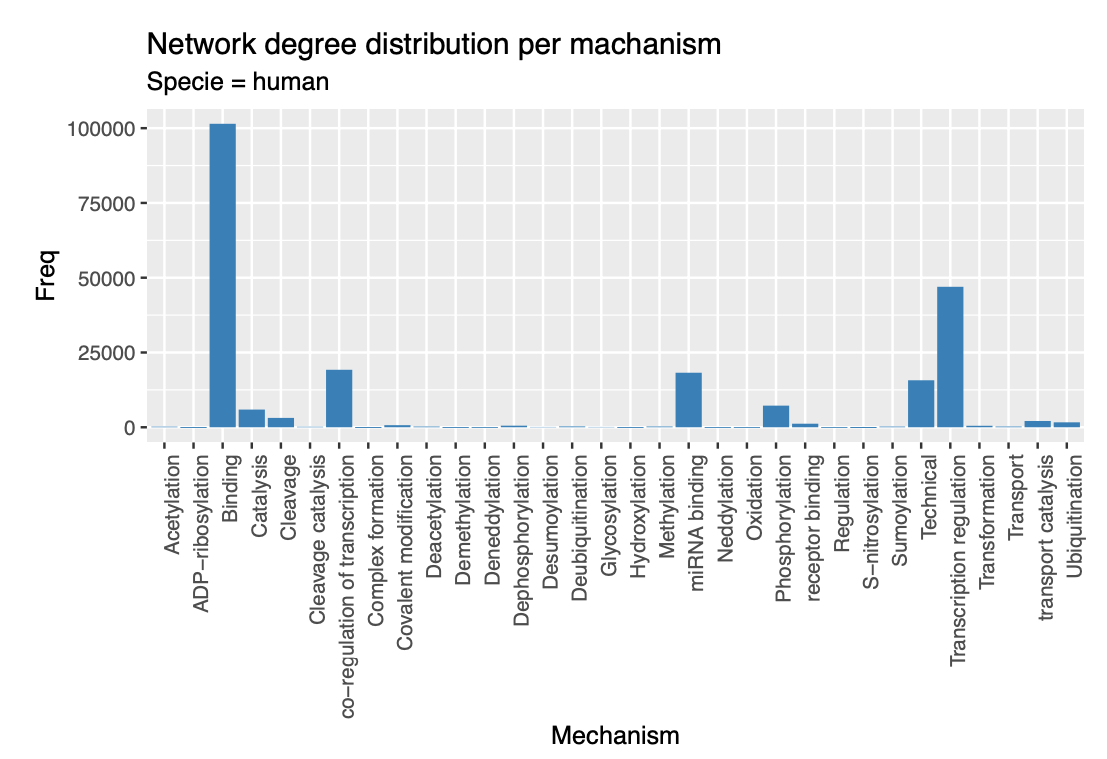
\includegraphics[width=\textwidth, height=\textheight, keepaspectratio]{Major Thesis/figures/eda/Degree_human.png}
            \caption{Histogram edge mechanism labels in MetaCore network for \textit{homo sapiens}}
    \end{subfigure}
    \hfill
    \begin{subfigure}{0.5\linewidth}
        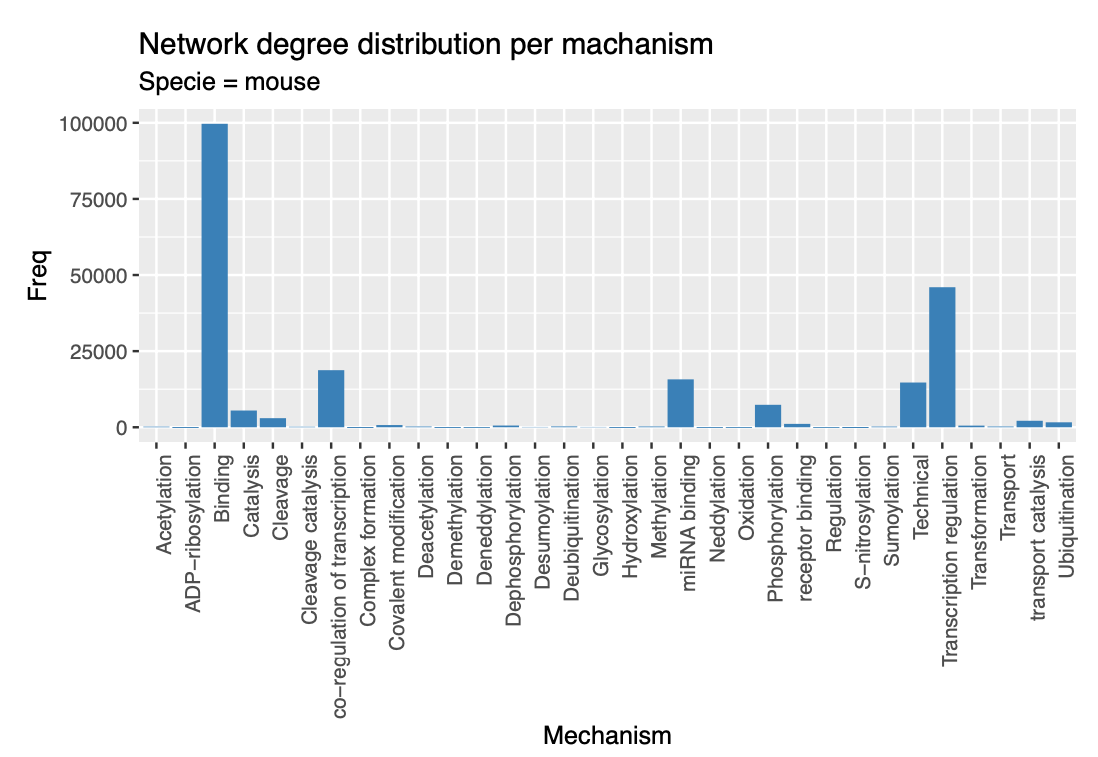
\includegraphics[width=\textwidth, height=\textheight, keepaspectratio]{Major Thesis/figures/eda/Degree_mice.png}
            \caption{Histogram edge mechanism labels in MetaCore network for \textit{mus musculus}}
    \end{subfigure}
    \caption{Mechanism labels for different species.}
    \label{img:suppl:degrees}
\end{figure}


\subsection{Extra Insight Results}
\label{section:suppl:results}
\subsubsection{IUT Component}
Showing top ranked (1st position) items across contrasts.
\begin{figure}[!htbp]
    \centering
    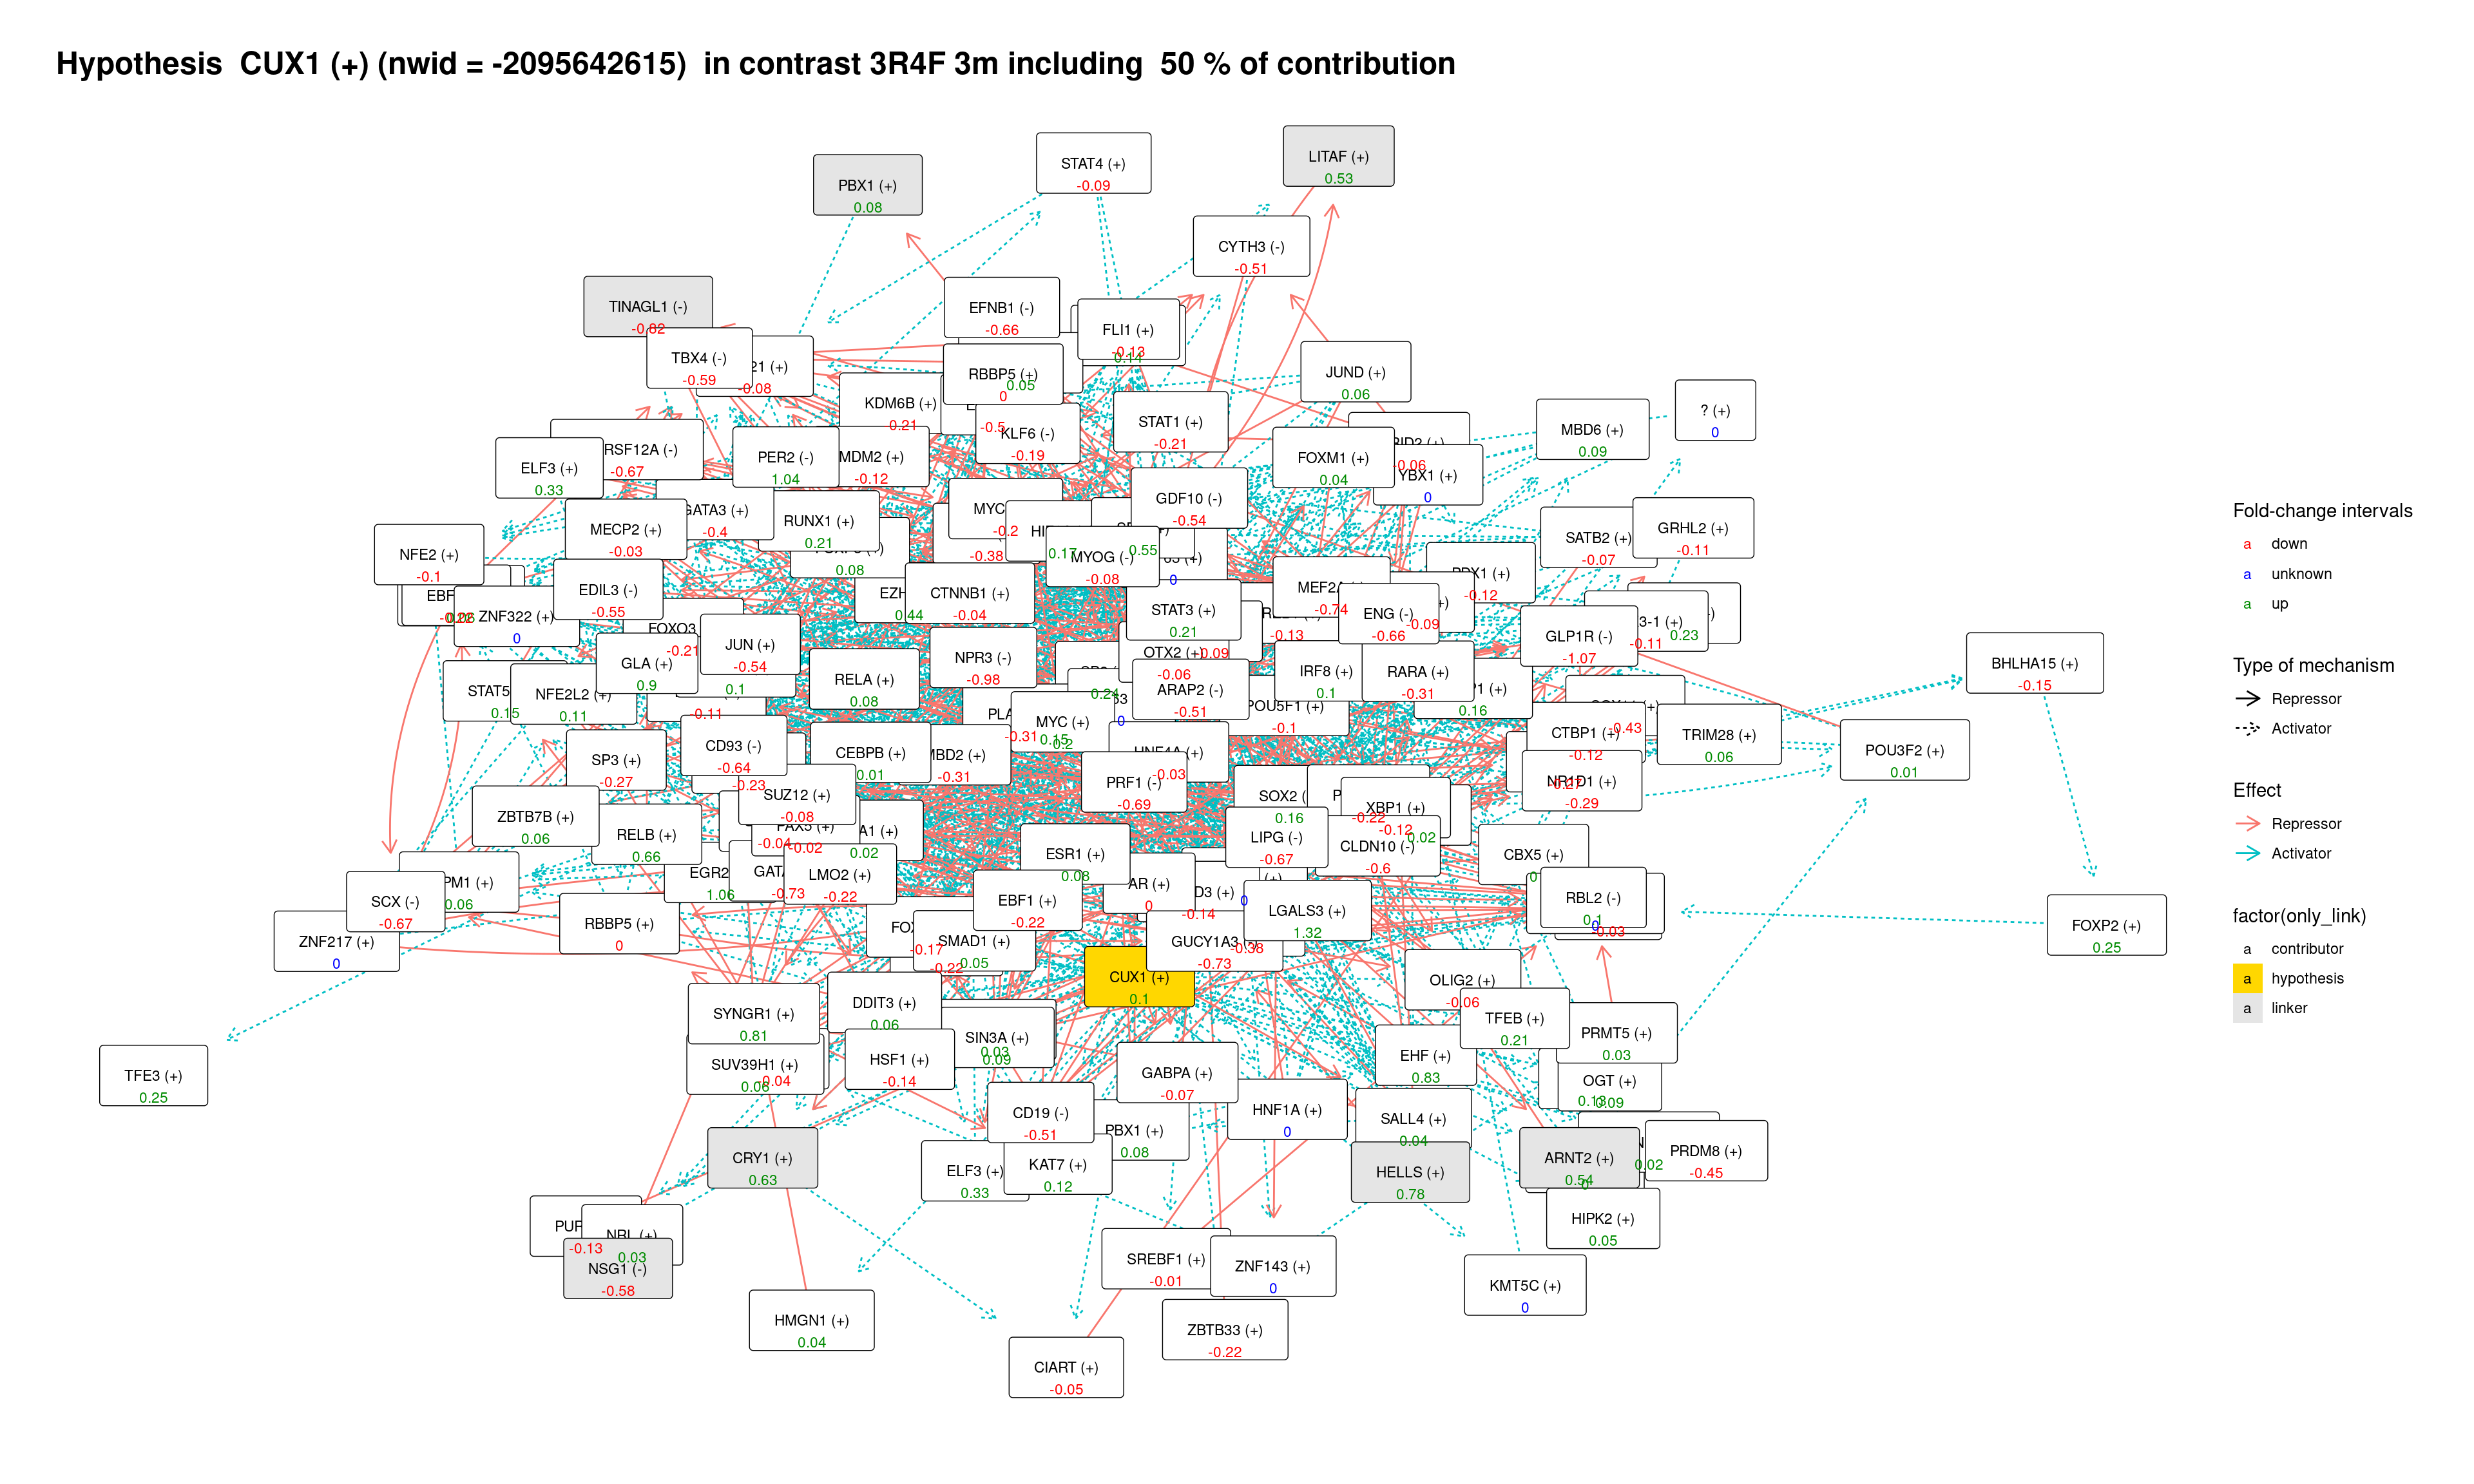
\includegraphics[width=\textwidth, height=\textheight, keepaspectratio]{Major Thesis/figures/iut/graph/3R4F3m50-CUX1.png}
    \caption{Interaction sub-network of the top DE ranked gene CUX1 (Cut Like Homeobox 1) at node 50\% contribution. SigNet run on 3R4F 3m contrast.}
\end{figure}

\begin{figure}[!htbp]
    \centering
    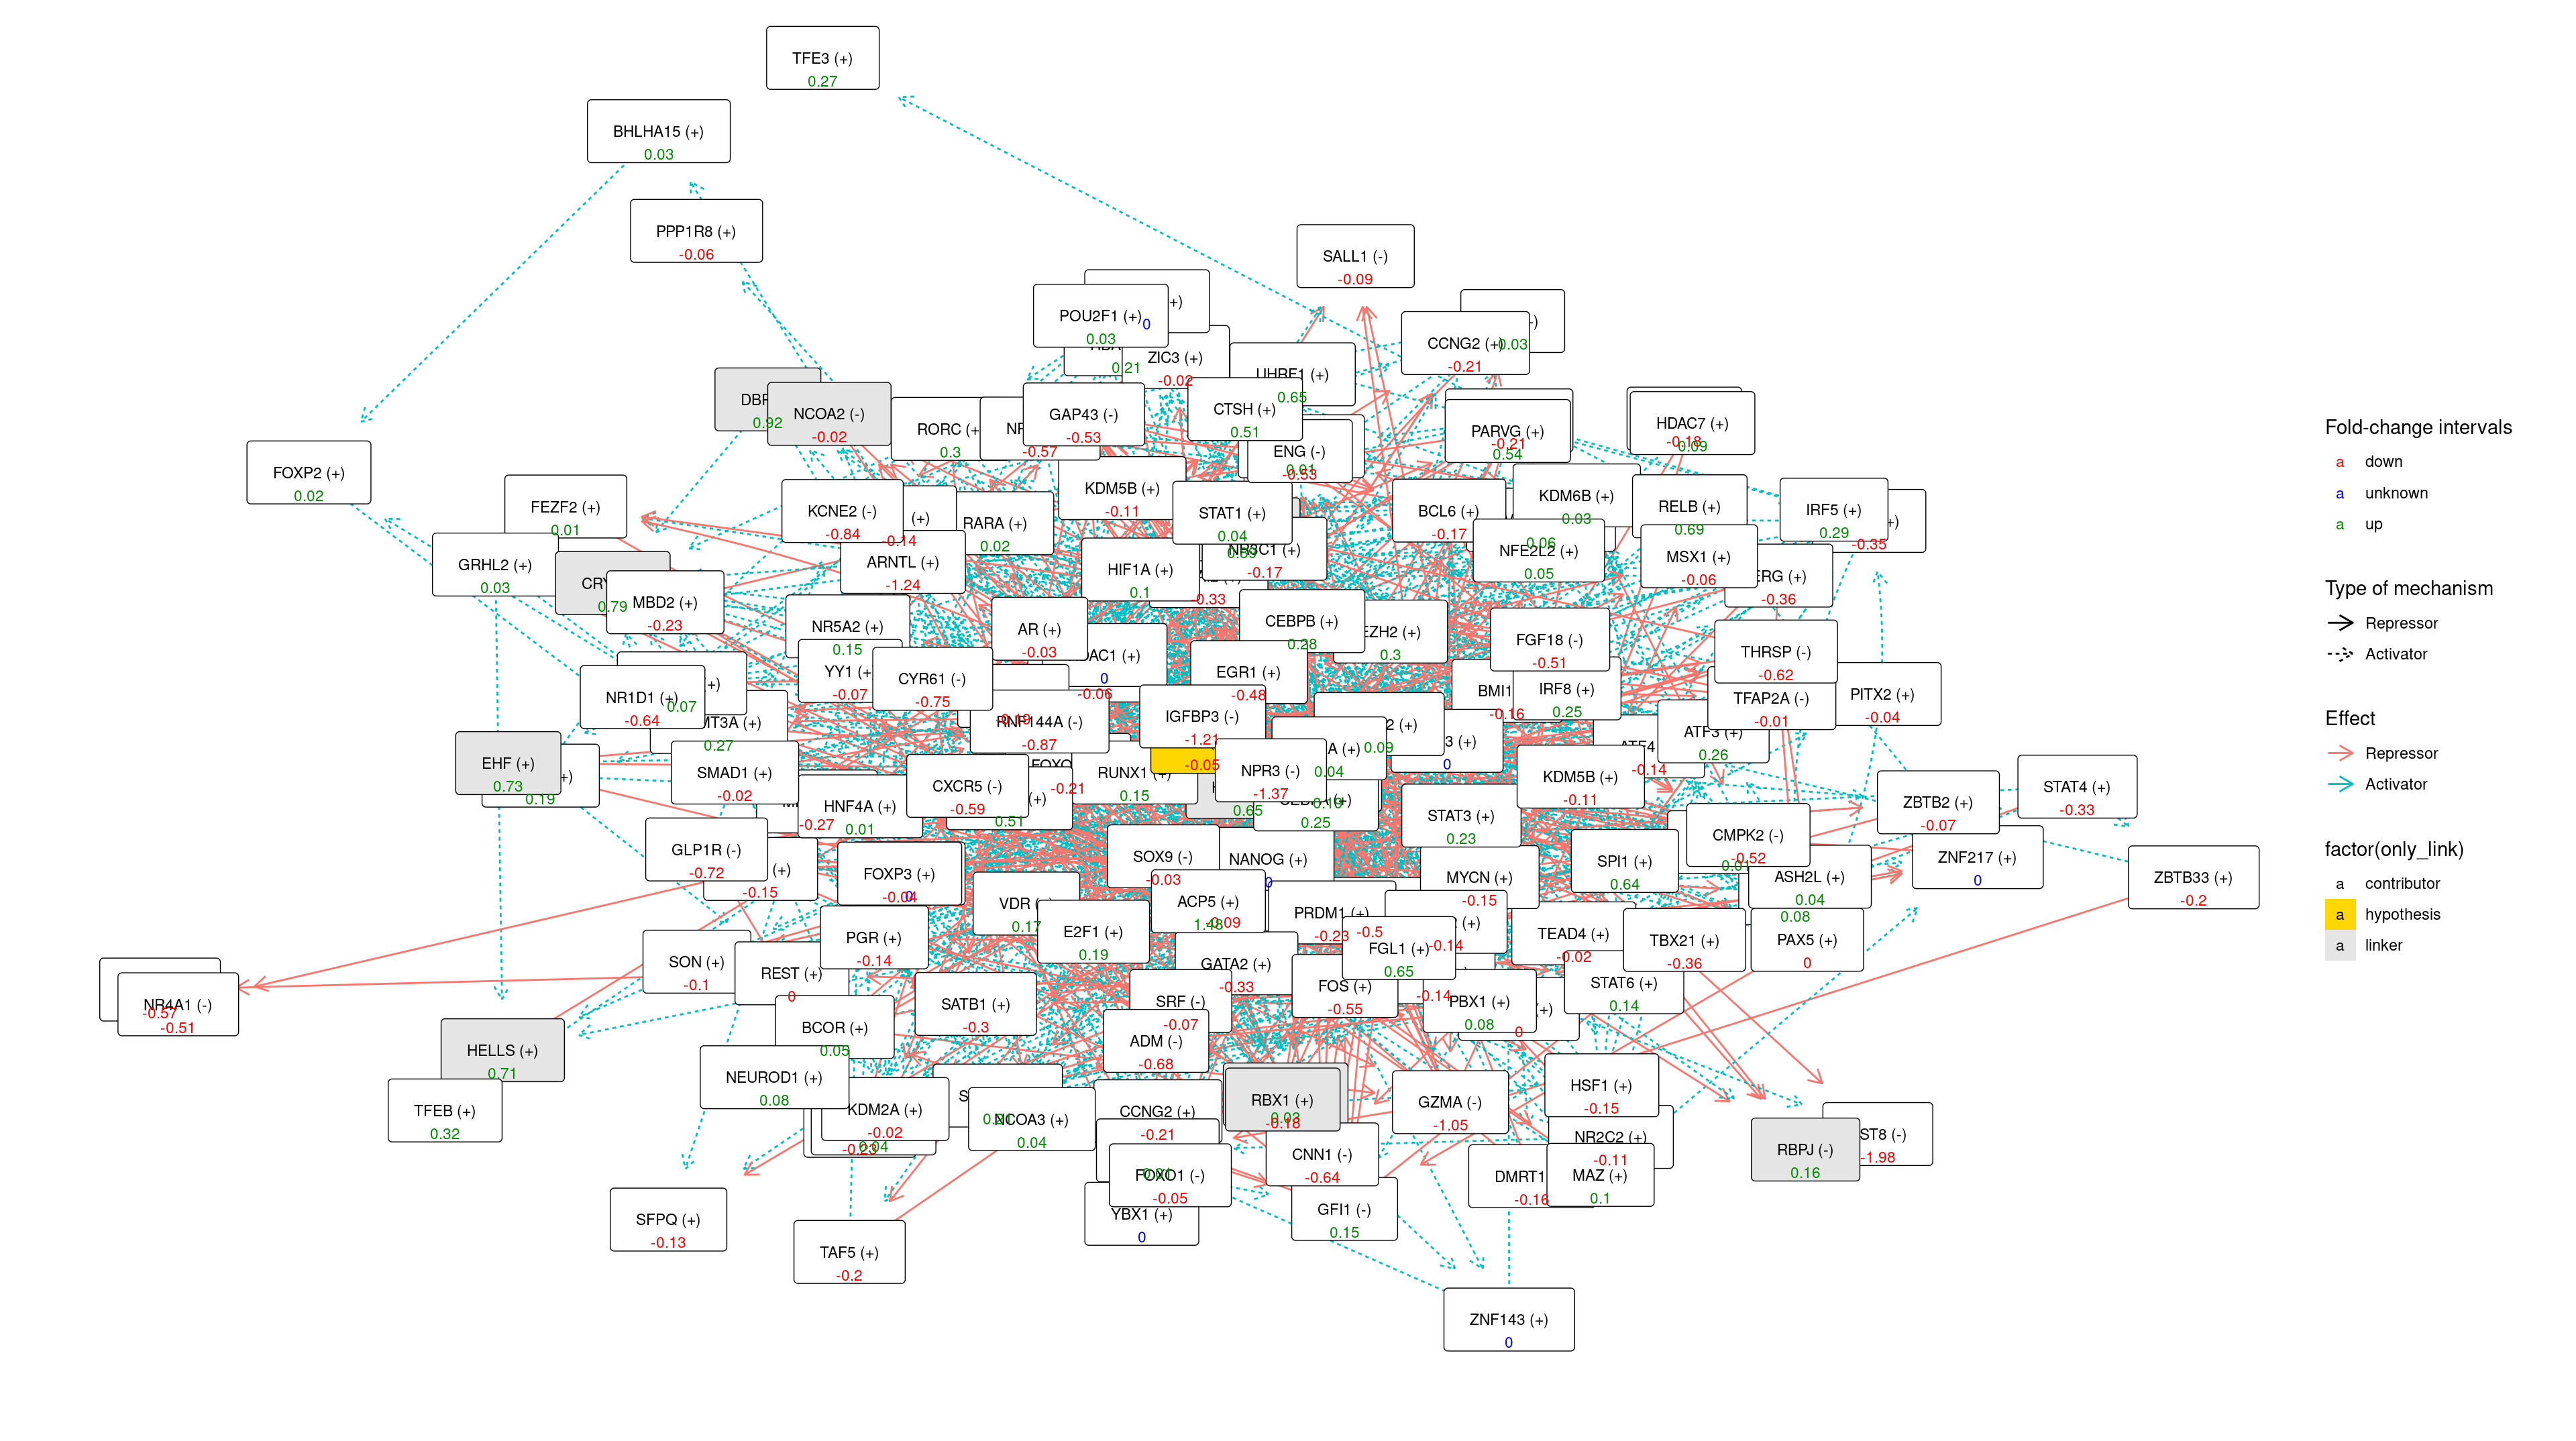
\includegraphics[width=\textwidth, height=\textheight, keepaspectratio]{Major Thesis/figures/iut/graph/3R4F4m50-SP1.png}
    \caption{Interaction sub-network of the top DE ranked gene SP1 (Sp1 Transcription Factor) at node 50\% contribution. SigNet run on 3R4F 4m contrast.}
\end{figure}

\begin{figure}[!htbp]
    \centering
    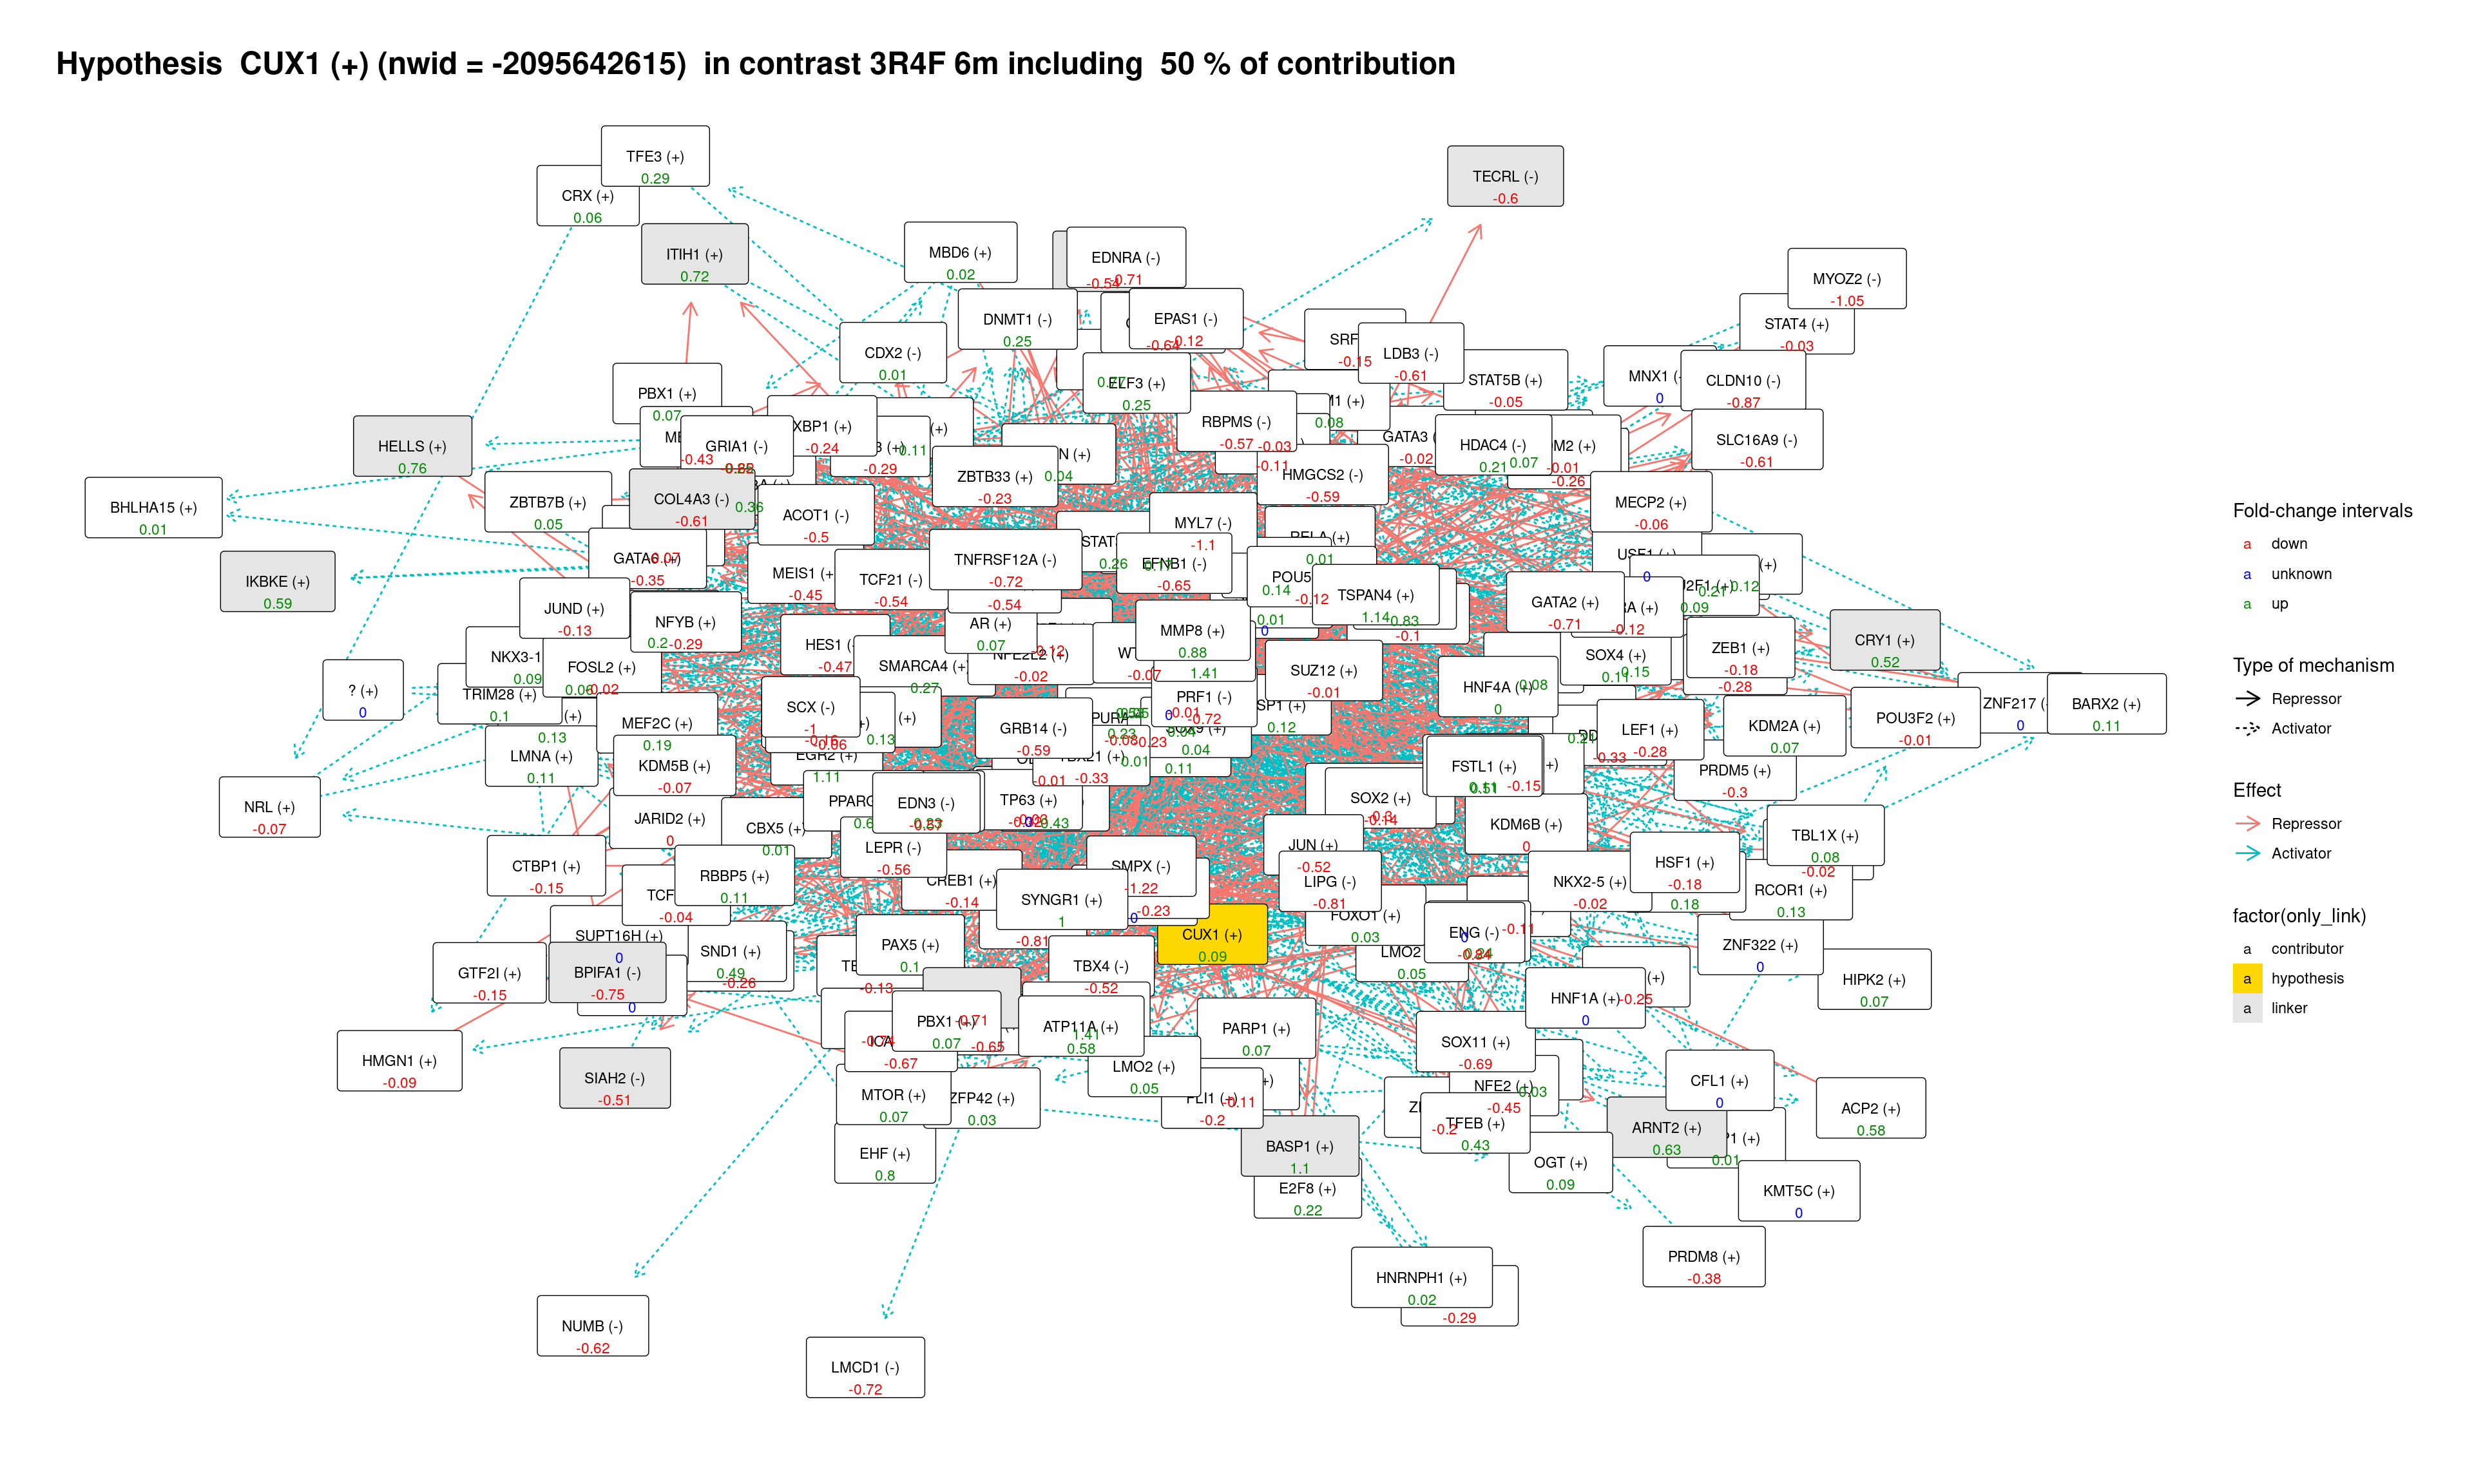
\includegraphics[width=\textwidth, height=\textheight, keepaspectratio]{Major Thesis/figures/iut/graph/3R4F46m50-CUX1.png}
    \caption{Interaction sub-network of the top DE ranked gene CUX1 (Cut Like Homeobox 1) at node 50\% contribution. SigNet run on 3R4F 6m contrast.}
\end{figure}


\begin{figure}[!htbp]
    \centering
    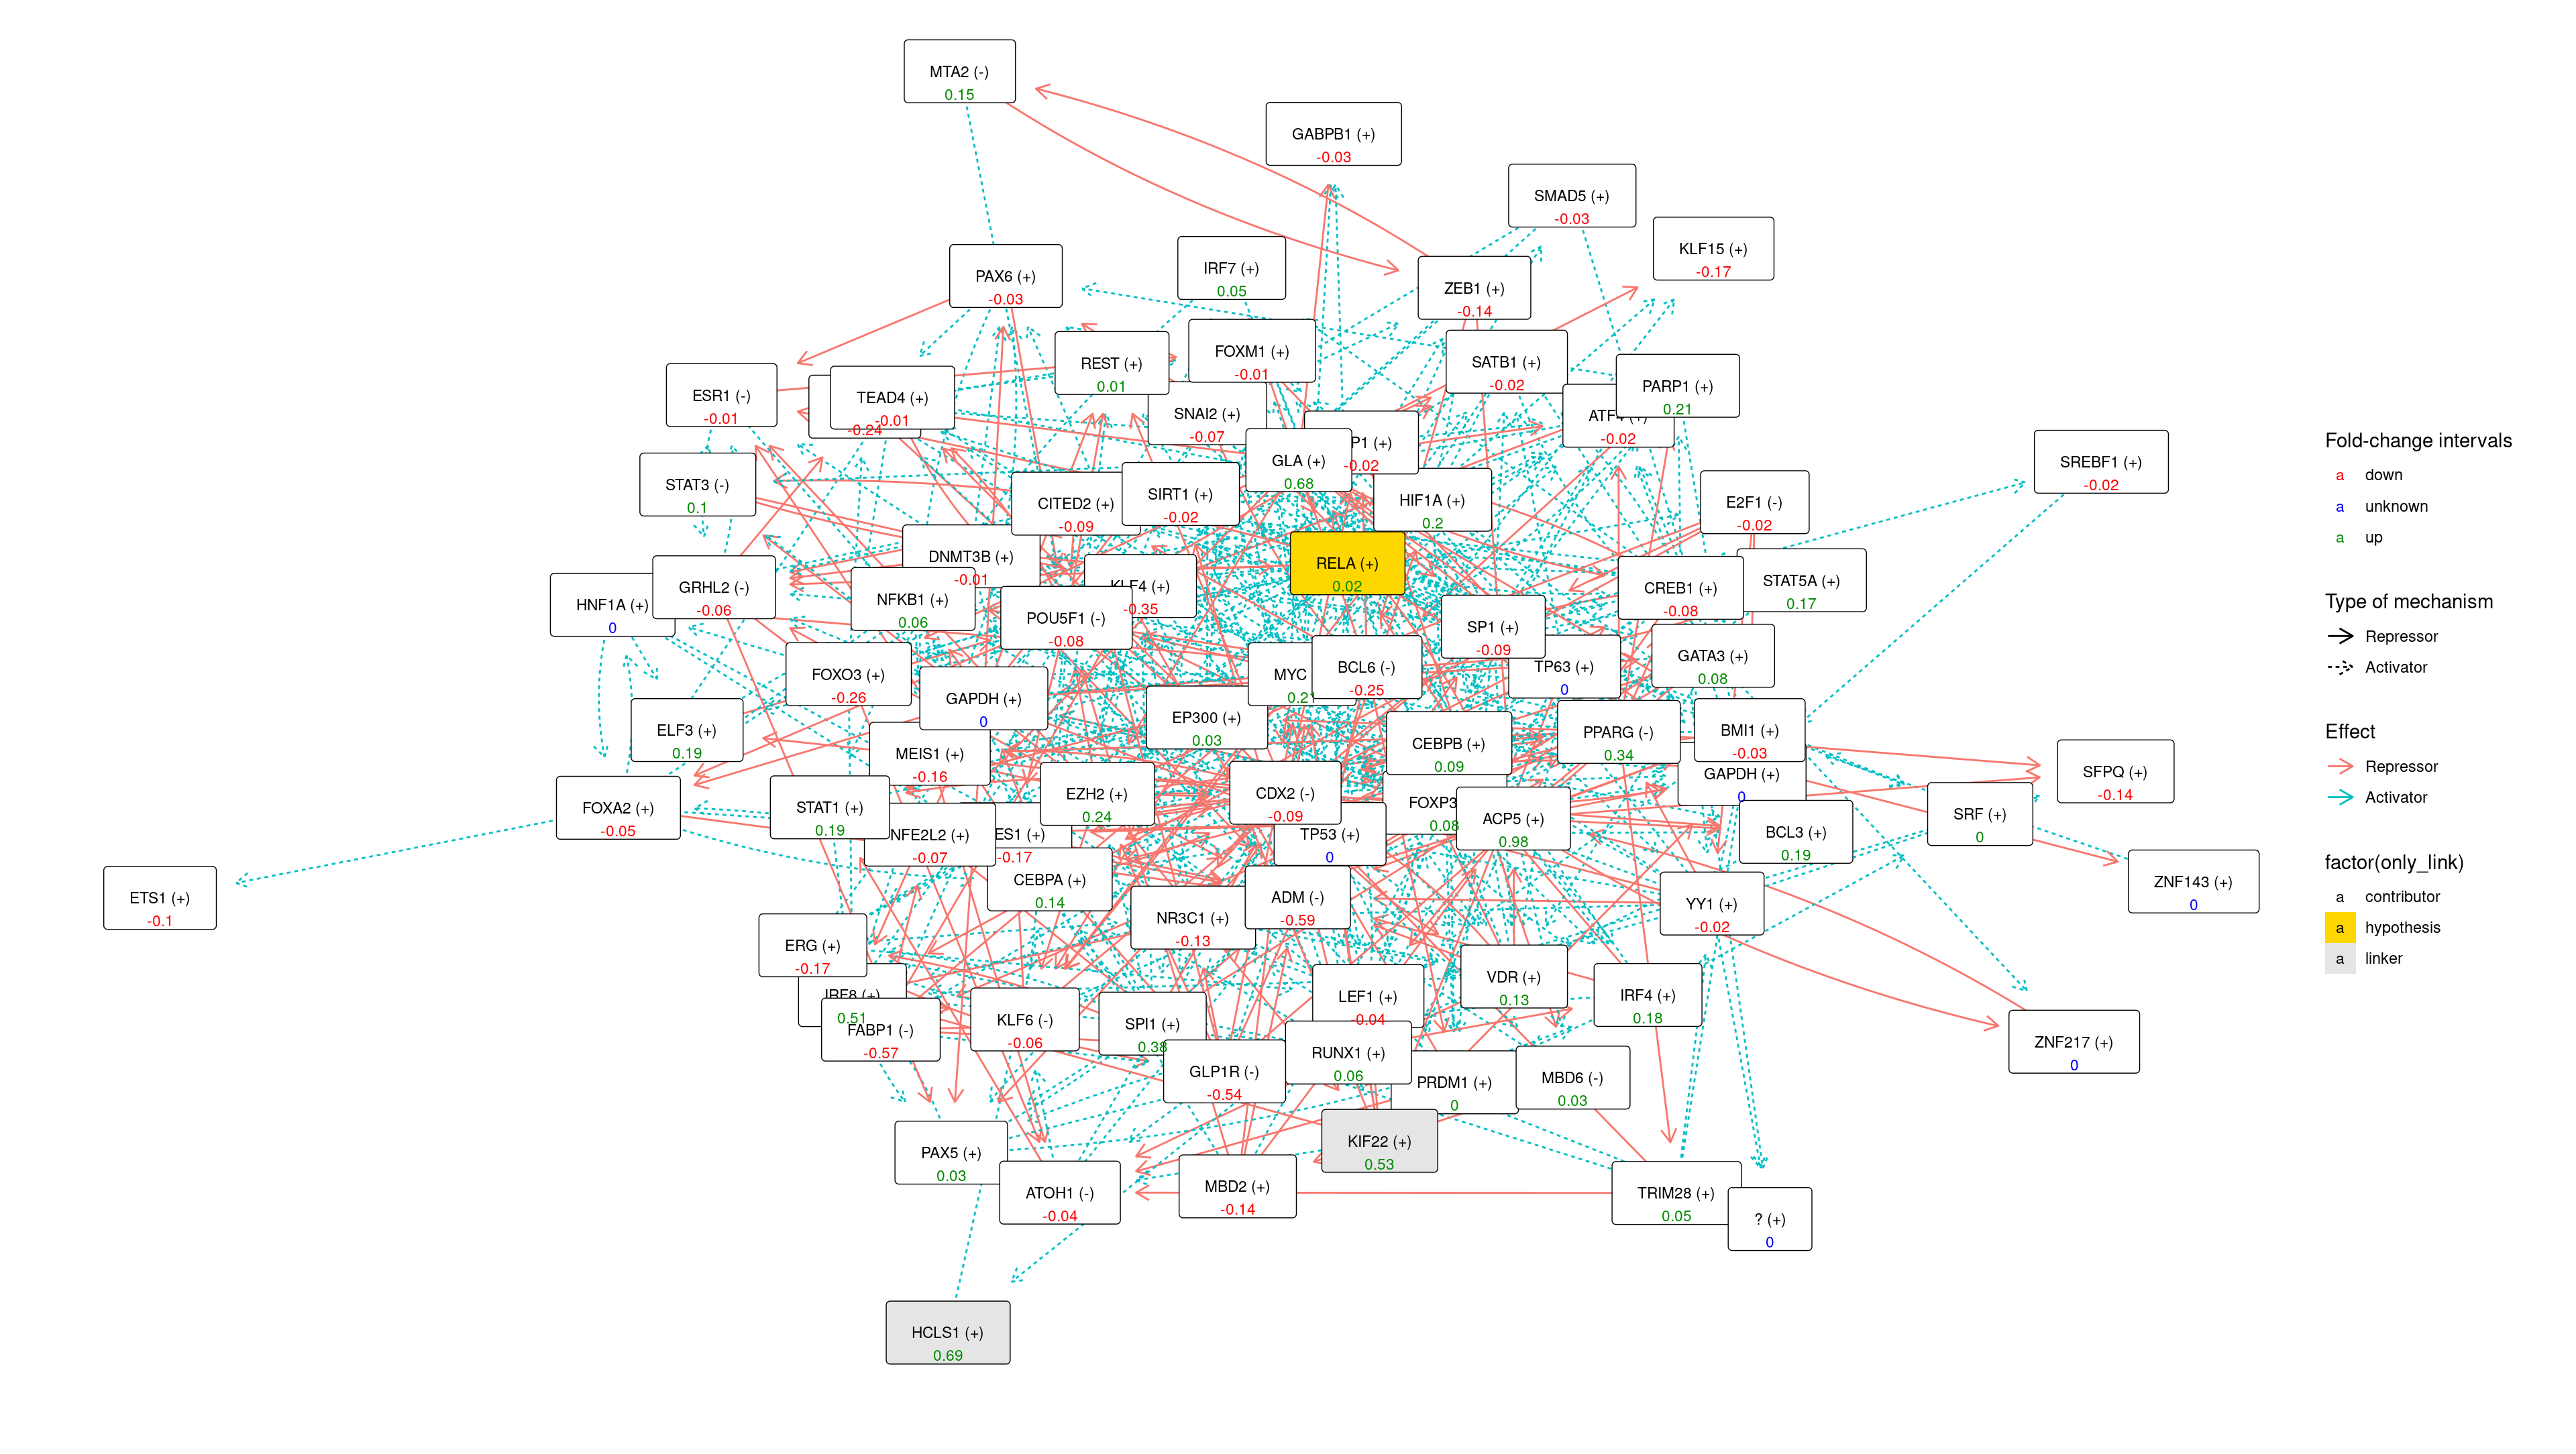
\includegraphics[width=\textwidth, height=\textheight, keepaspectratio]{Major Thesis/figures/iut/graph/CESS4m50-RELA.png}
    \caption{Interaction sub-network of the top DE ranked gene RELA (RELA Proto-Oncogene, NF-KB Subunit) at node 50\% contribution. SigNet run on CESS 4m contrast.}
\end{figure}

\begin{figure}[!htbp]
    \centering
    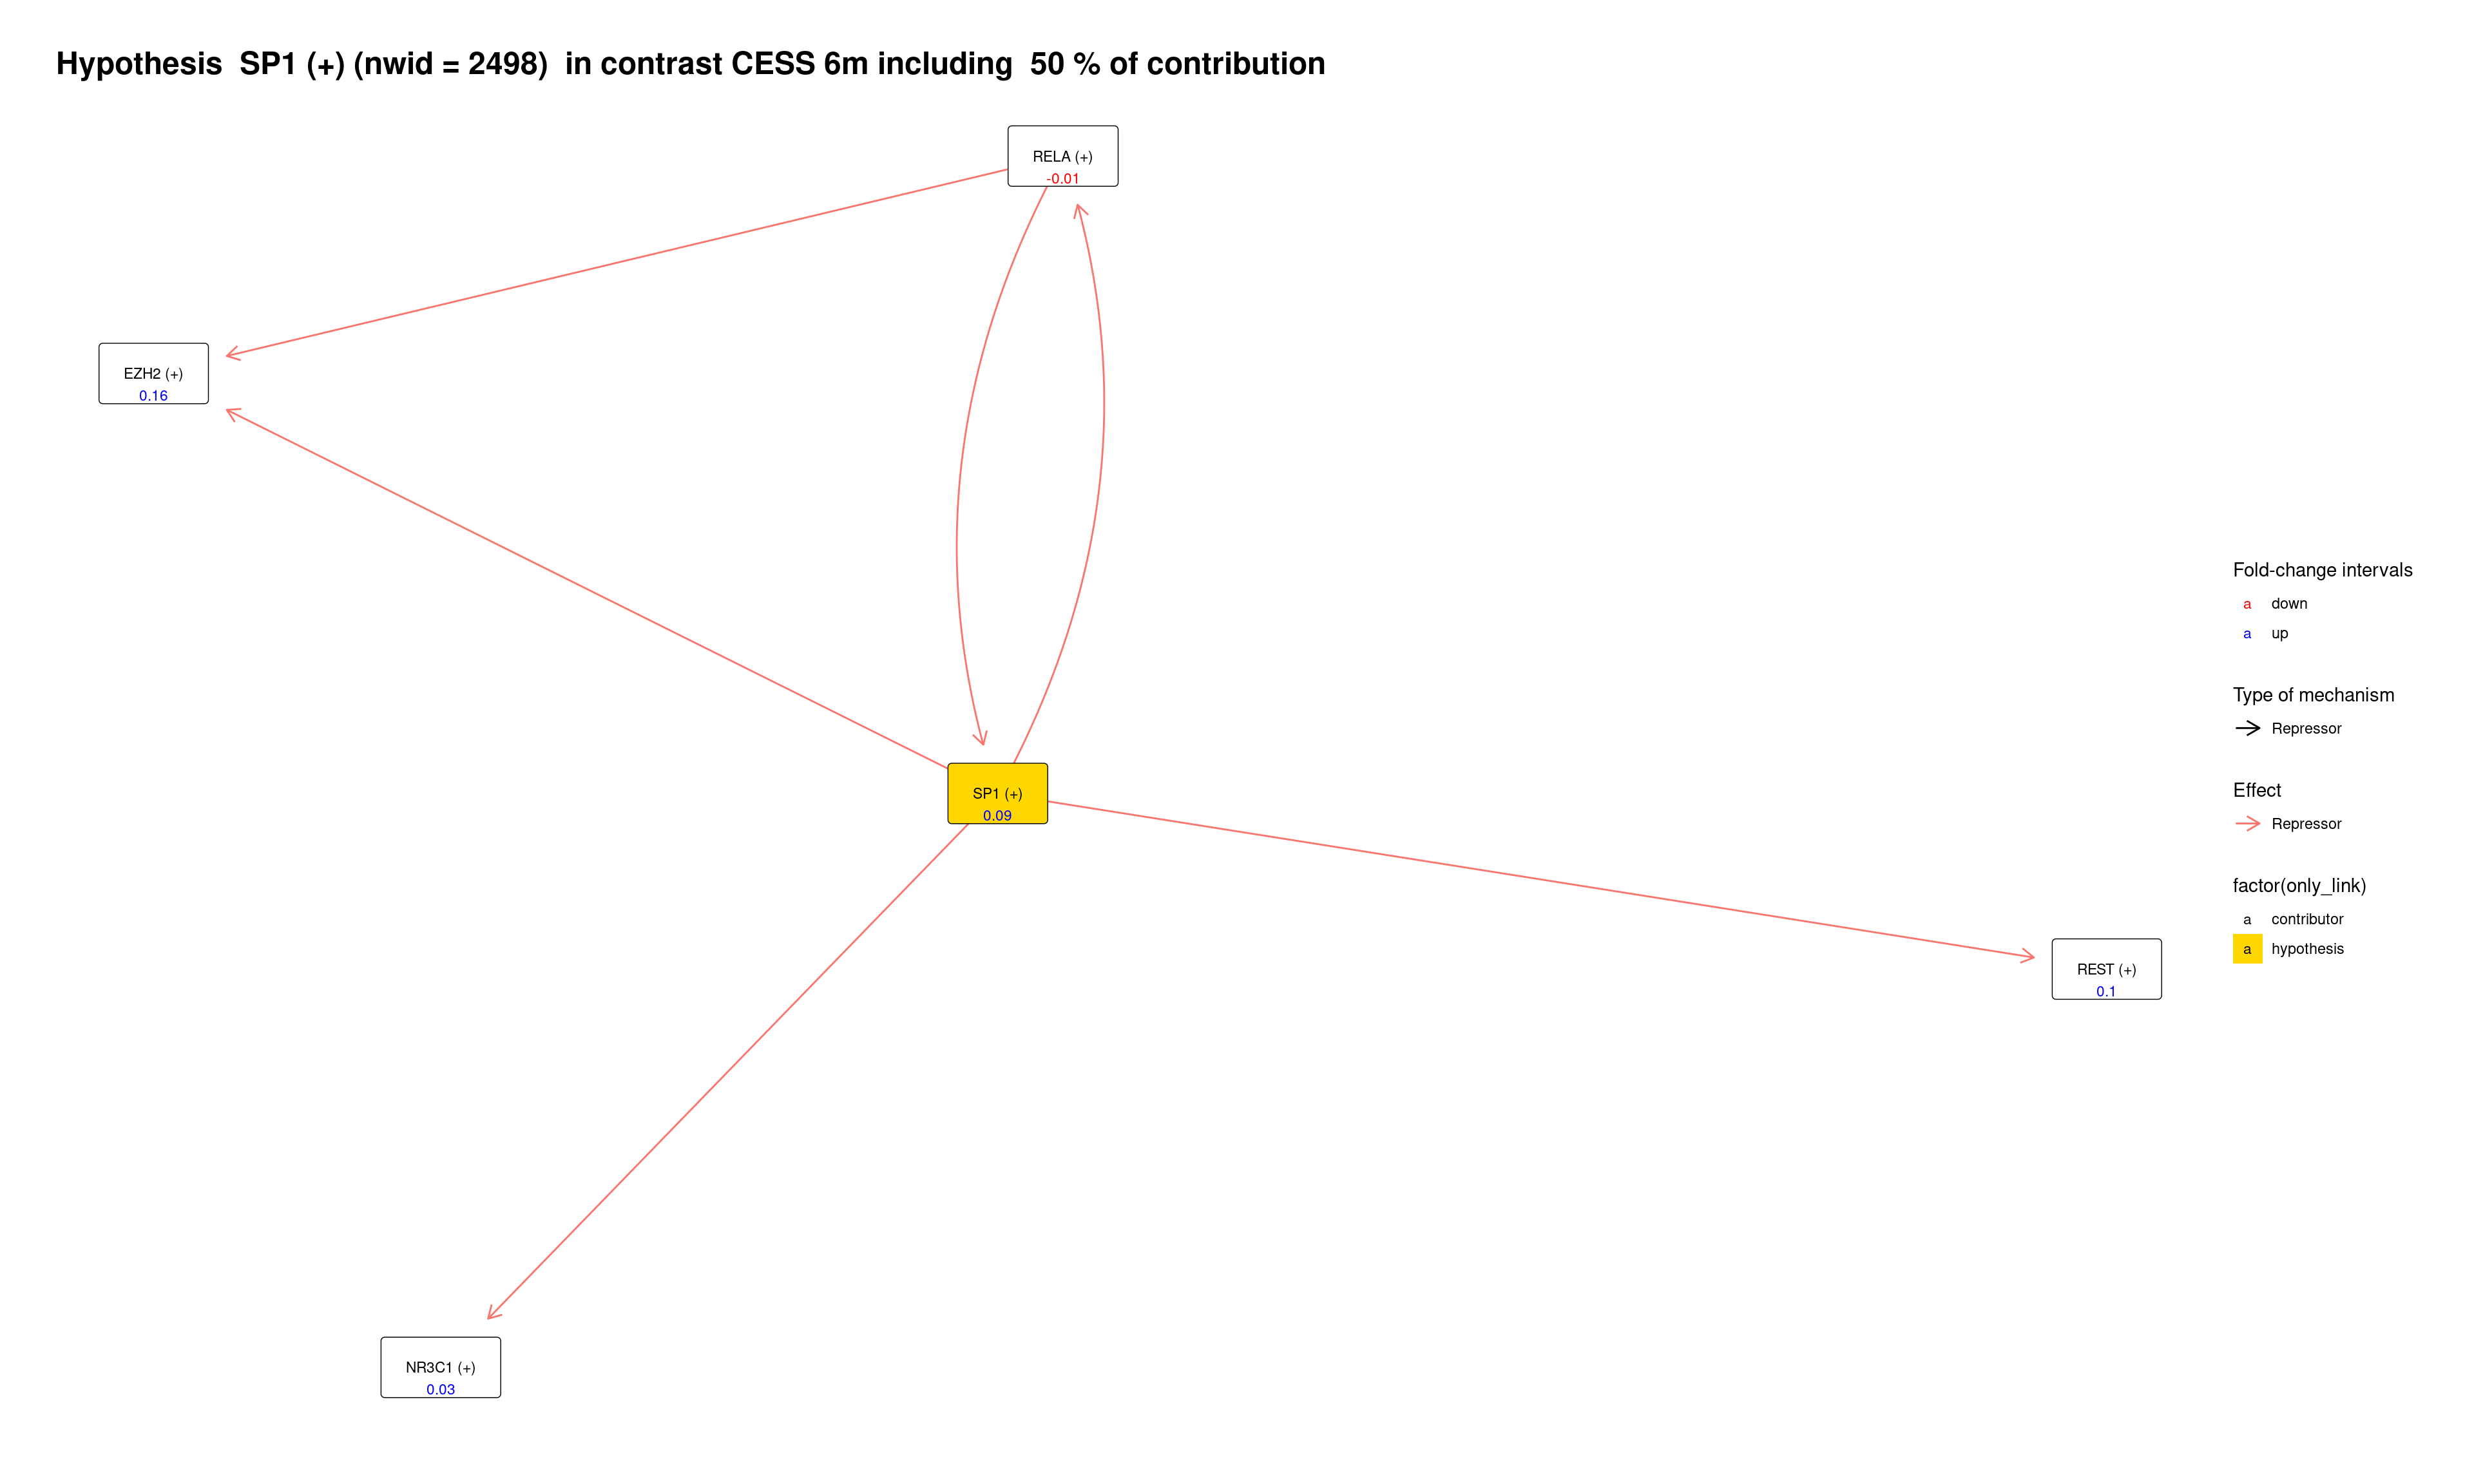
\includegraphics[width=\textwidth, height=\textheight, keepaspectratio]{Major Thesis/figures/iut/graph/CESS6m50-SP1.png}
    \caption{Interaction sub-network of the top DE ranked gene SP1 (Sp1 Transcription Factor) at node 50\% contribution. SigNet run on CESS 6m contrast.}
\end{figure}

\begin{figure}[!htbp]
    \centering
    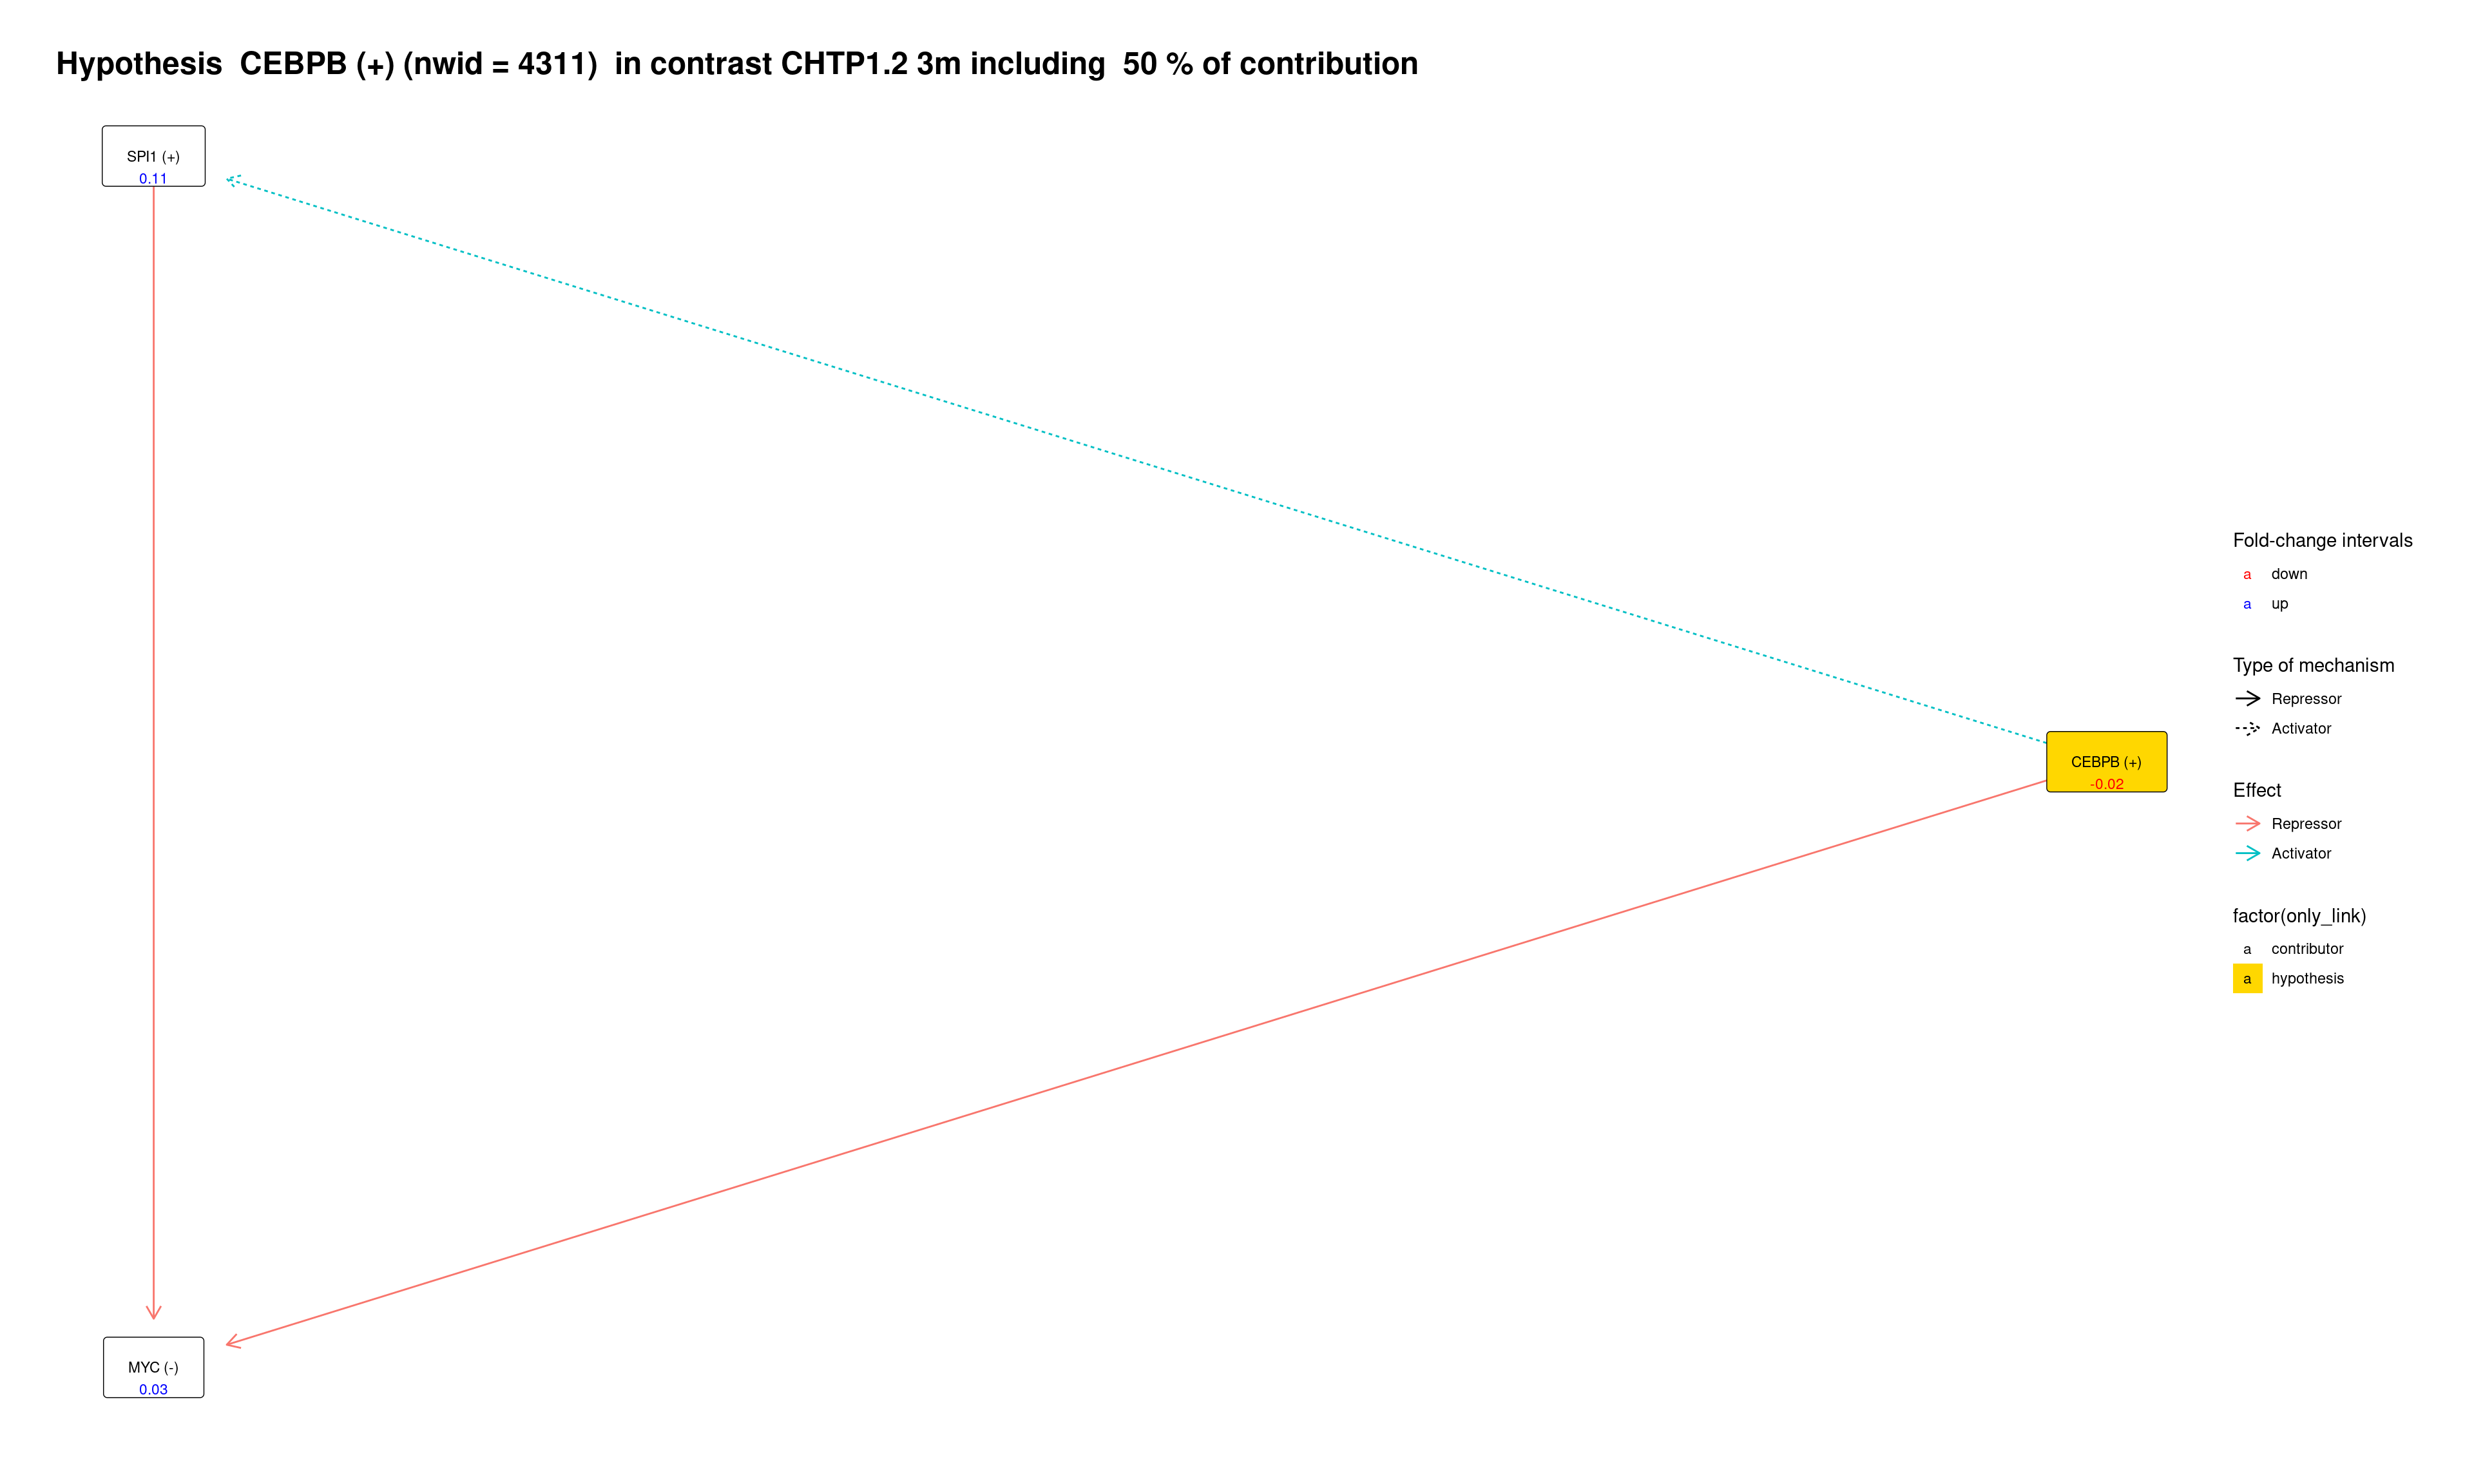
\includegraphics[width=\textwidth, height=\textheight, keepaspectratio]{Major Thesis/figures/iut/graph/CHTP3m-CEBPB.png}
    \caption{Interaction sub-network of the top DE ranked gene CEBPB (CCAAT Enhancer Binding Protein Beta) at node 50\% contribution. SigNet run on CHTP 3m contrast.}
\end{figure}

\begin{figure}[!htbp]
    \centering
    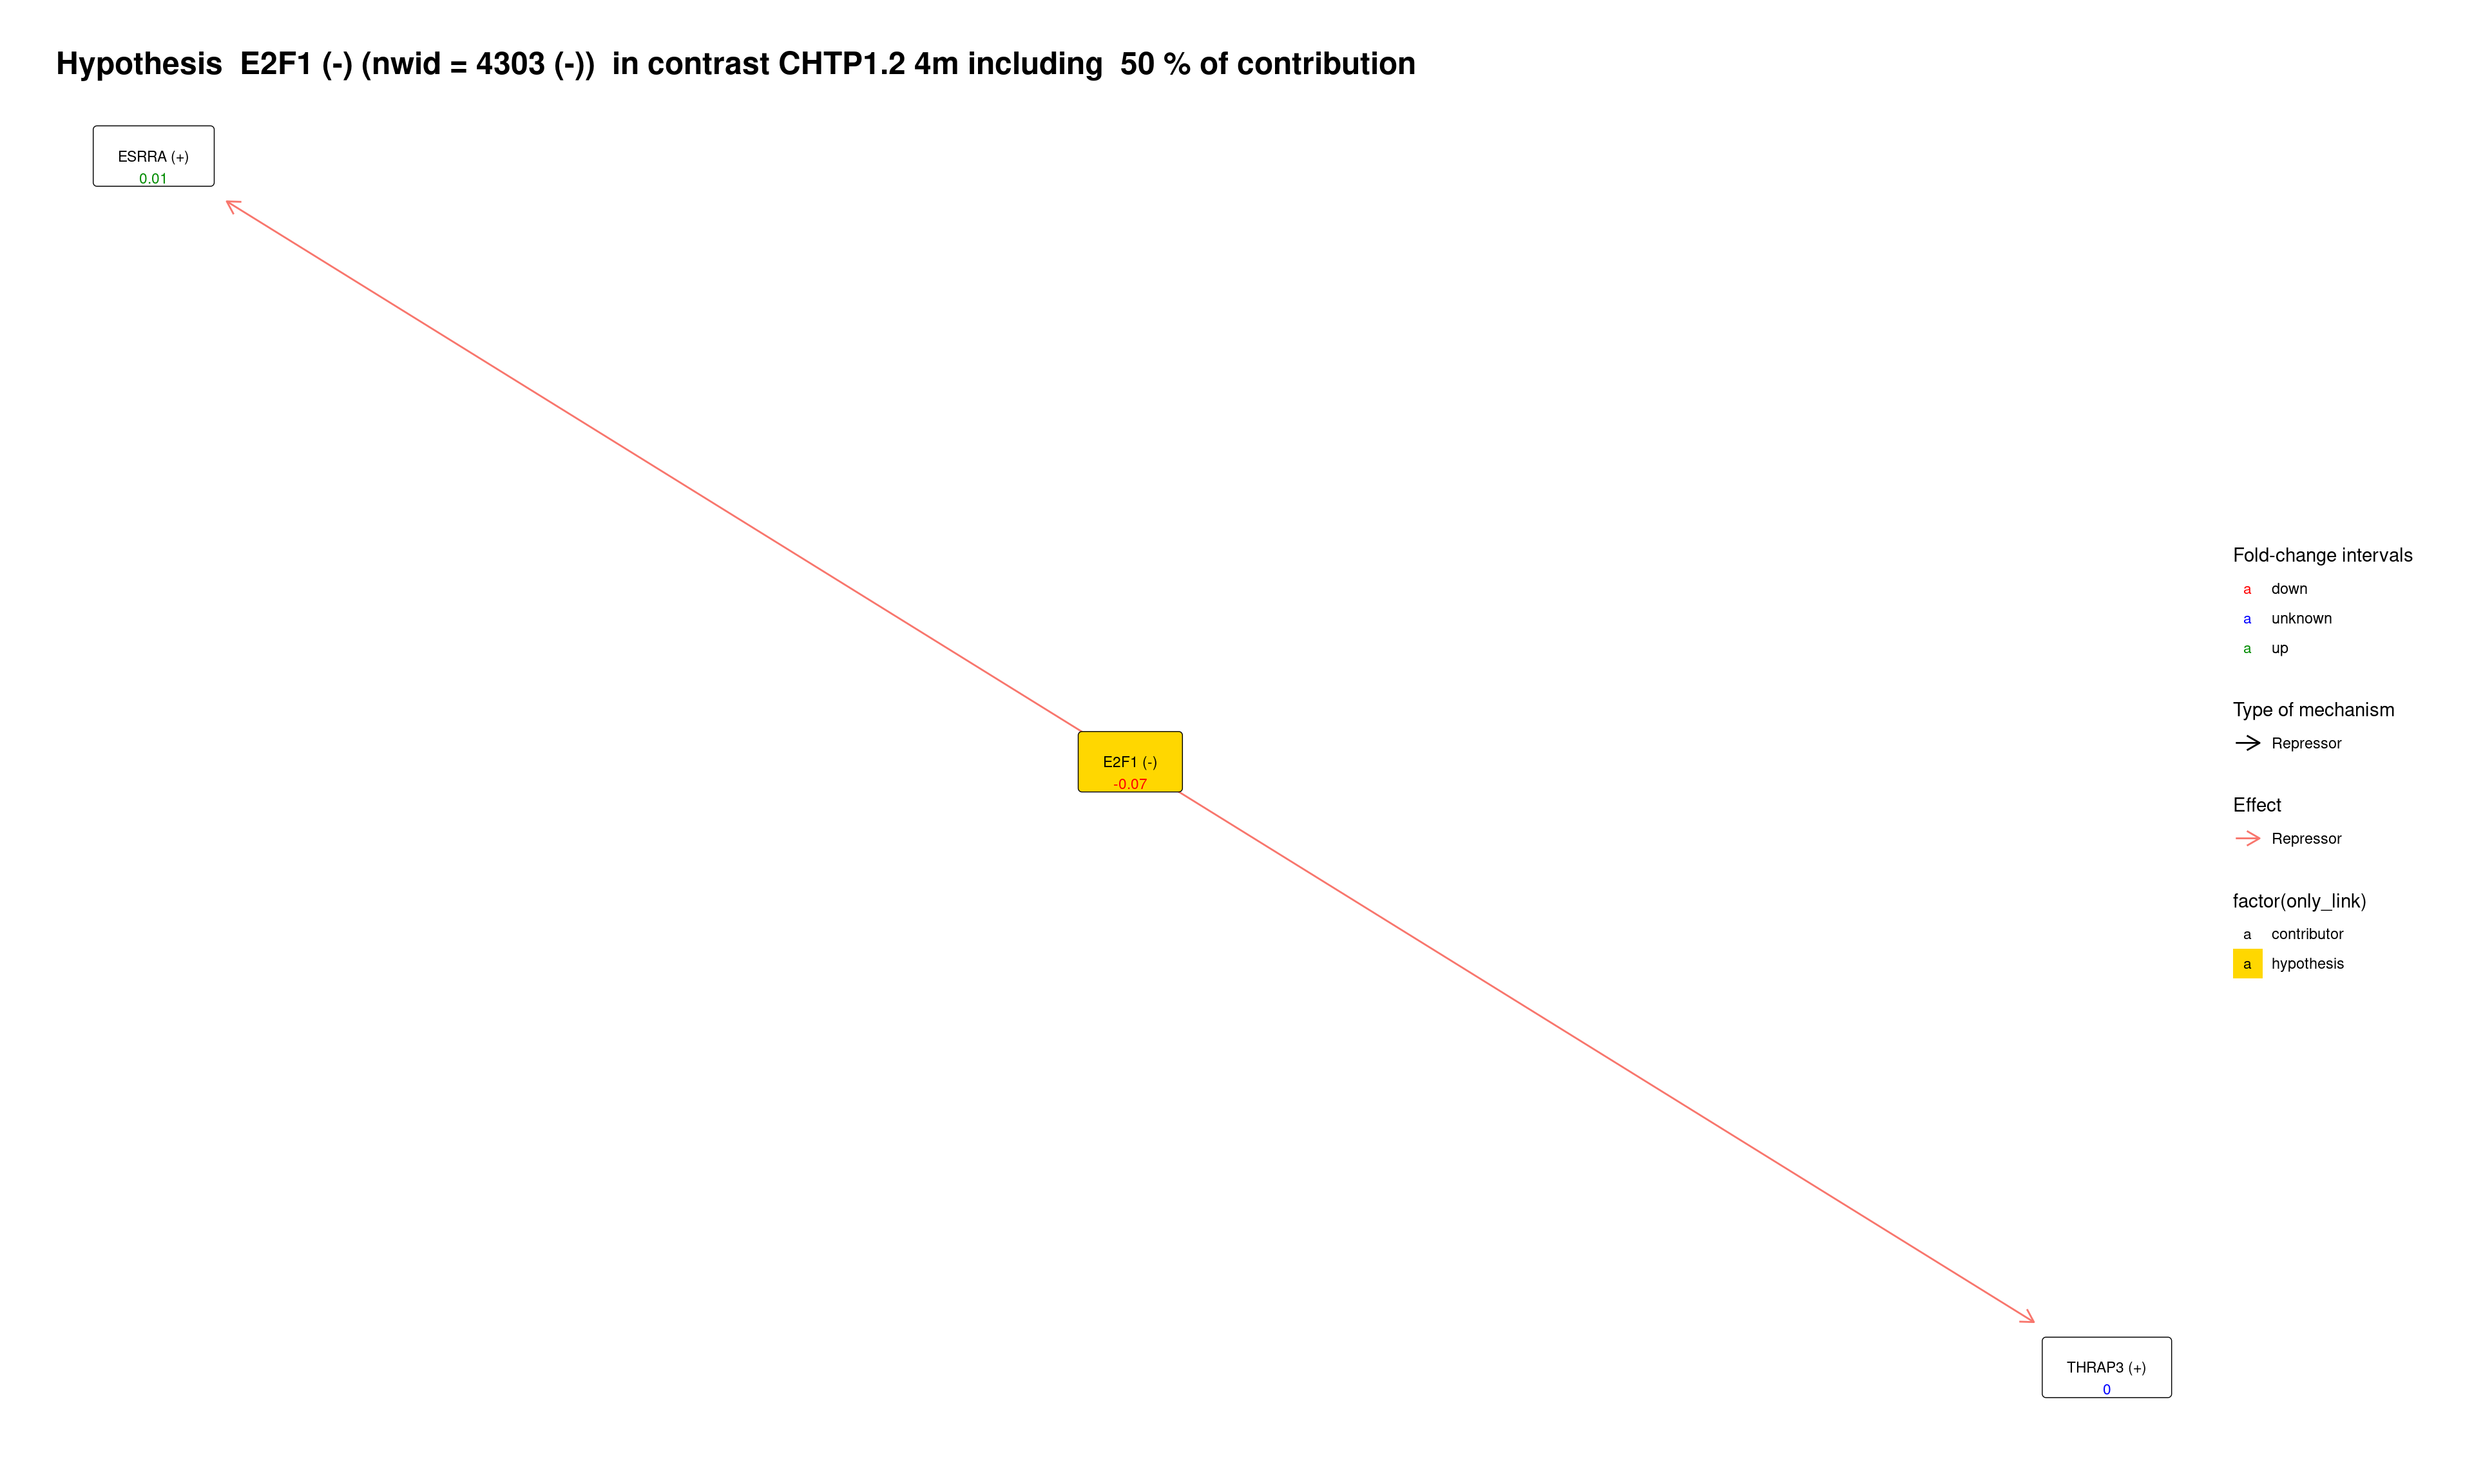
\includegraphics[width=\textwidth, height=\textheight, keepaspectratio]{Major Thesis/figures/iut/graph/CHTP4m-E2F1.png}
    \caption{Interaction sub-network of the top DE ranked gene E2F1 (E2F Transcription Factor 1) at node 50\% contribution. SigNet run on CHTP 4m contrast.}
\end{figure}

\begin{figure}[!htbp]
    \centering
    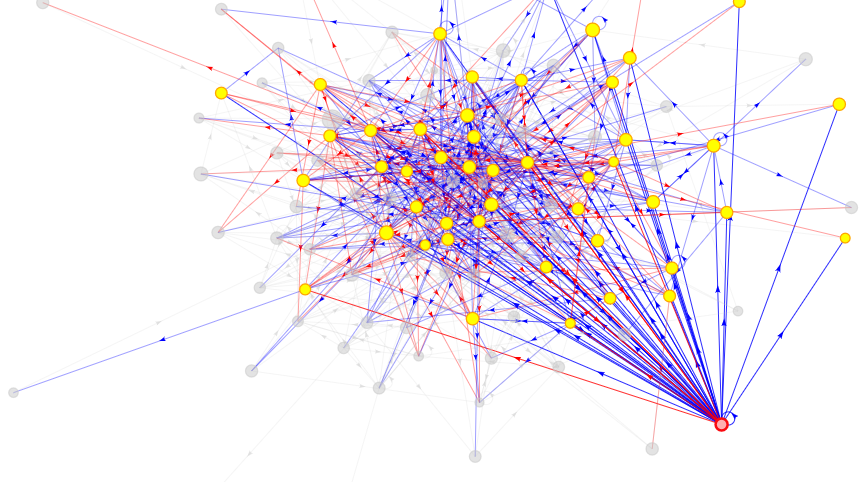
\includegraphics[width=\textwidth, height=\textheight, keepaspectratio]{Major Thesis/figures/iut/graph/i3R4F-overall.png}
    \caption{Interactive version for Interaction sub-network of the top DE ranked gene CUX1 (Cut Like Homeobox 1) at node 50\% contribution. SigNet run on 3R4F 3m contrast.}
    \label{section:suppl:results:3R4F-interactive}
\end{figure}

\begin{figure}[!htbp]
    \centering
    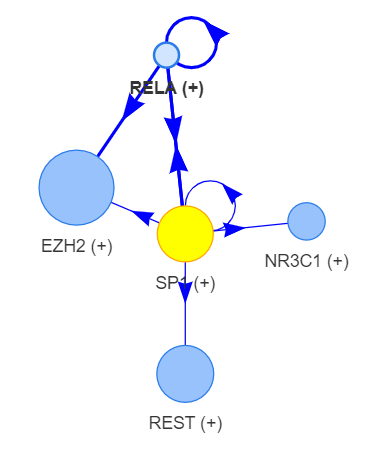
\includegraphics[width=0.5\textwidth, height=\textheight, keepaspectratio]{Major Thesis/figures/iut/graph/iCESS6m50-SP1.png}
    \caption{Interactive version for Interaction sub-network of the top DE ranked gene SP1 (Sp1 Transcription Factor) at node 50\% contribution. SigNet run on CESS 6m contrast.}
    \label{section:suppl:results:cess-interactive}
\end{figure}

\subsubsection{DES-nA Component}
\subfile{desna-collapsed-tableDEG.tex}

\FloatBarrier

\subsection{CEL Files treatment}
CMAP2 \cite{Subramanian2017AProfiles} relates gene expression to drug targets. It disposes of raw-data “.CEL” formatted files generated by scanning a single Affymetrix microarray.

An instance table is also available to provide the relation between CEL files and lab-specific data.

CEL files were downloaded from CMAP2’ webpage via R scripting. The Instances table is also available in the same site and serves as coordinator of the case-control comparison, as well as for correctly labelling the cases.

IDMAPGen is an R package function developed at PMI. The procedure of the internal calculations held within is out of the scope of this project. It requires the CEL formatted objects as input and a coordination file, as the Instances table.

The label name is composed by collapsing together the cmap\_name, molar concentration, and cell type, and is used to tag the classes. For the CEL files naming, note the perturbation column includes a large identification number and a second label after a full stop. These are the names of the CEL files. The controls corresponding to each perturbation are formed by the same identification number and each label available in the control column. E.g. perturbation = 123.H1, control = .A1.B2.C3, then the CEL files for the case is 123.H1 and for its controls are 123.A1, 123.B2 and 123.C3. 

Due to package unavailability and compatibility issues with our current version of R Studio, only HT\_HG-U133A array derived cases have been considered which accounts for the 65\% of the total CEL files available in CMAP. The procedure delivers 1991 test cases to use as benchmark which we consider sufficient.

The calculation of the final objects results in a list of cases, each containing at least the fold-change of each analyzed gene and its p-value. The naming of each gene has been supported by external BioConductor library frmavecs, Affymetrix reader functions and biomaRt homo\_sapiens\_ensembl dataset \footnote{https://cran.r-project.org/web/packages/biomartr/index.html}.
\label{section:suppl:bench}

\subsection{Algorithms further explanations}
\label{section:suppl:algorithms}

\subsubsection{SigNet}
\label{section:suppl:algorithms-signet}
By inputting gene expression data which we filter, a causal graph is built from it, taking a known interaction network (INN) as reference. All the edges present in the graph numerically indicate the kind of edge from which we derive the named mechanism: “1” for activation, “-1” for repression and “0” for unknown cases.

For the construction, each node X is duplicated, creating an “activated” version (X+) and a repressed version (X-). For node interaction definition, e.g. X and Y in INN, if there is an activation edge from X to Y, then (X+) —> (Y+), and (X-) —> (Y-) are linked. Conversely, if there’s a repression factor, it yields (X+) —> (Y-) and (X-) —> (Y+). For unknown cases, edges are converted to pairs of edges with both activation and repression effects.

The resulting graph is then divided into a bipartite graph, splitting hypothesis from downstream phenotypical items. All 6 scoring systems include the shortest path (SP) value in their arithmetic. One of the parameters to optimize SP is reachability limit, which treats a node as \textit{unreachable } after a default threshold of 20 jumps.

(Return to main text \ref{back:section:signet})

\paragraph{Default Scoring systems}
Where AFC = Absolute Fold-Change, SP = Shortest Path, reach(A, B) = A reaches B (True = 1, False = 0)

\begin{center}
    $NormalWeight(A) = \sum{b\ in\ signature} AFC(B) \times sign(SP(\neg B, A) - SP(B, A))$ \\    
    $PowerWeight(A) = \sum{b\ in\ signature} AFC(B)^{SP(B, A)}$ \\
    $Lambda(A) = \frac{\sum{b\ in\ signature} reach(A, B)}{cardinal(signature)} + \sum{b\ in\ signature} \frac{SP(B, A)}{cardinal(signature) \times MAXDISTANCE}$ \\
\end{center}


\subsubsection{MARINa Scoring}
\label{section:suppl:algorithms-marina}
As described in \cite{Lefebvre2010ACenters}, results use DETOR score for \emph{differentially expressed target odds ratio}:
\begin{center}
    $DETOR_{TF_{i}} &= \frac{GS_{i}^{LE}/RS_{i}^{LE}}{GS_{i}/RS_{i}}$
\end{center}

where $GS_{i}^{LE}$ and $RS_{i}^{LE}$ are the number of genes before the leading edge in GSEA for the gene set (or regulon) and for the reference set, whereas $GS_{i}$ and $RS_{i}$ are the sizes of the gene set and the reference set.